% Source :
%    https://tex.stackexchange.com/a/540432/6880

\documentclass{article}
\usepackage[margin=0.5in]{geometry}% need more space
\usepackage[utf8]{inputenc}
\usepackage{tikz}
\usepackage{pgfplots}
\usetikzlibrary{intersections}
\usepackage{amsmath}
\usepackage{amssymb}
\usepackage{setspace}
\usepackage{relsize}
\usepackage{sectsty}
\usepackage{array}
\usepackage{tabularx}
\usepackage{makecell}
\usepackage{cellspace}
\usepackage{multirow}
\setcellgapes{7.5pt}
\setlength\cellspacetoplimit{7.5pt}
\setlength\cellspacebottomlimit{7.5pt}

\setlength\parindent{0pt}
\newcommand{\form}[1]{\textbf{\textsf{#1}}}
\onehalfspacing

\begin{document}
\begin{center}
    \makegapedcells
    \setlength\tabcolsep{10pt}
    \begin{tabular}{|c|c|c|c|c|}
        \hline
        \multicolumn{2}{|c|}{\form{Discriminant}} & $\Delta = b^2-4ac > 0$ & $\Delta = b^2-4ac = 0$ & $\Delta = b^2-4ac < 0$\\
        \hline
        \multicolumn{2}{|c|}{\form{Solutions}}
        & \parbox[c]{120pt}{\centering \form{2 racines simples}\\ $x = x_1 = \mathlarger{\frac{-b-\sqrt{\Delta}}{2a}}$\\ ou\\ $x = x_2 = \mathlarger{\frac{-b+\sqrt{\Delta}}{2a}}$}
        & \parbox[c]{120pt}{\centering \form{Une racine double}\\ $x = x_0 = -\mathlarger{\frac{b}{2a}}$} & \form{Pas de solutions dans} $\mathbb{R}$ \\
        \hline
        \multicolumn{2}{|c|}{\form{Forme factorisée}} & $a(x-x_1)(x-x_2)$ & $a(x-x_0)^2$
        & \parbox[c]{120pt}{\form{Pas de forme factorisée dans} $\mathbb{R}$}\\
        \hline
        \raisebox{-40pt}[0pt][0pt]{\form{Graphe}} & $a > 0$ & 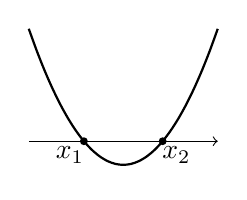
\begin{tikzpicture}[baseline=(current bounding box.center)]
                                                        \def\zoom{0.6}
                                                        \coordinate (O) at (0,0);
                                                        \draw [name path=left] ({-\zoom*2},0)--(O);
                                                        \draw [->, name path=right] (O)--({\zoom*2},0);
                                                        \draw [thick, domain=-1.2:1.2, smooth, variable=\x, name path=P] plot (\x, {\zoom*2*\x*\x-.3});
                                                        \path [name intersections={of=left and P, by=X1}];
                                                        \path [name intersections={of=right and P, by=X2}];
                                                        \fill [black] (X1) circle (0.05) node [xshift=-5, yshift=-5]{$x_1$};
                                                        \fill [black] (X2) circle (0.05) node [xshift=5, yshift=-5]{$x_2$};
                                                    \end{tikzpicture}
                                                    & 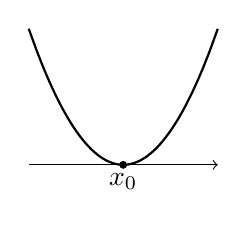
\begin{tikzpicture}[baseline=(current bounding box.center)]
                                                        \def\zoom{0.6}
                                                        \coordinate (O) at (0,0);
                                                        \draw [name path=left] ({-\zoom*2},0)--(O);
                                                        \draw [->, name path=right] (O)--({\zoom*2},0);
                                                        \draw [thick, domain=-1.2:1.2, smooth, variable=\x, name path=P] plot (\x, {\zoom*2*\x*\x});
                                                        \path [name intersections={of=left and P, by=X0}];
                                                        \fill [black] (X0) circle (0.05) node [yshift=-6]{$x_0$};
                                                    \end{tikzpicture}
                                                    & 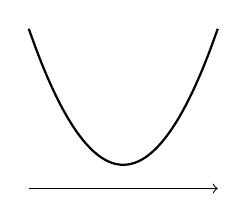
\begin{tikzpicture}[baseline=(current bounding box.center)]
                                                        \def\zoom{0.6}
                                                        \coordinate (O) at (0,0);
                                                        \draw [name path=left] ({-\zoom*2},0)--(O);
                                                        \draw [->, name path=right] (O)--({\zoom*2},0);
                                                        \draw [thick, domain=-1.2:1.2, smooth, variable=\x, name path=P] plot (\x, {\zoom*2*\x*\x+.3});
                                                    \end{tikzpicture}\\
                                                    \cline{2-5}
                                    & $a < 0$ & 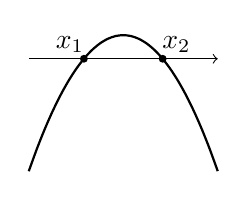
\begin{tikzpicture}[baseline=(current bounding box.center)]
                                                    \def\zoom{0.6}
                                                    \coordinate (O) at (0,0);
                                                    \draw [name path=left] ({-\zoom*2},0)--(O);
                                                    \draw [->, name path=right] (O)--({\zoom*2},0);
                                                    \draw [thick, domain=-1.2:1.2, smooth, variable=\x, name path=P] plot (\x, {-\zoom*2*\x*\x+.3});
                                                    \path [name intersections={of=left and P, by=X1}];
                                                    \path [name intersections={of=right and P, by=X2}];
                                                    \fill [black] (X1) circle (0.05) node [xshift=-5, yshift=5]{$x_1$};
                                                    \fill [black] (X2) circle (0.05) node [xshift=5, yshift=5]{$x_2$};
                                                \end{tikzpicture}
                                                & 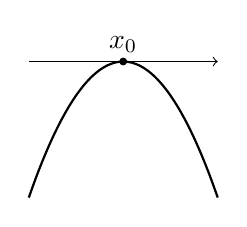
\begin{tikzpicture}[baseline=(current bounding box.center)]
                                                    \def\zoom{0.6}
                                                    \coordinate (O) at (0,0);
                                                    \draw [name path=left] ({-\zoom*2},0)--(O);
                                                    \draw [->, name path=right] (O)--({\zoom*2},0);
                                                    \draw [thick, domain=-1.2:1.2, smooth, variable=\x, name path=P] plot (\x, {-\zoom*2*\x*\x});
                                                    \path [name intersections={of=left and P, by=X0}];
                                                    \fill [black] (X0) circle (0.05) node [yshift=6]{$x_0$};
                                                \end{tikzpicture}
                                                & 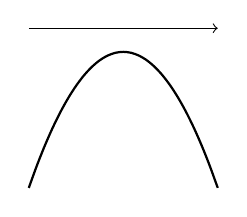
\begin{tikzpicture}[baseline=(current bounding box.center)]
                                                    \def\zoom{0.6}
                                                    \coordinate (O) at (0,0);
                                                    \draw [name path=left] ({-\zoom*2},0)--(O);
                                                    \draw [->, name path=right] (O)--({\zoom*2},0);
                                                    \draw [thick, domain=-1.2:1.2, smooth, variable=\x, name path=P] plot (\x, {-\zoom*2*\x*\x-.3});
                                                \end{tikzpicture}\\
        \hline
        \multirow{2}*{\form{Signe}} & $a > 0$ & ~ & ~ & ~\\\cline{2-5} & $a < 0$ & ~ & ~ & ~\\
        \hline
        \multirow{2}*{\form{Variations}} & $a > 0$ & \multicolumn{3}{c|}{~}\\\cline{2-5} & $a < 0$ & \multicolumn{3}{c|}{~}\\
        \hline
    \end{tabular}{}
    \label{tab:recap}
\end{center}
\end{document}
